\documentclass[12pt,a4paper]{article}
\usepackage[utf8]{inputenc}
\usepackage{amsmath}
\usepackage{amsfonts}
\usepackage{amssymb}
\usepackage{geometry}
\usepackage{graphicx}
\geometry{margin=1in}

\title{CENG499 Homework 3 Report}
\author{Name: Adilhan Çetin \\ Number: 2580421}

\begin{document}

\maketitle

\section*{Question 1}

\subsection*{a)}

\begin{figure}[hbt!]
    \centering
    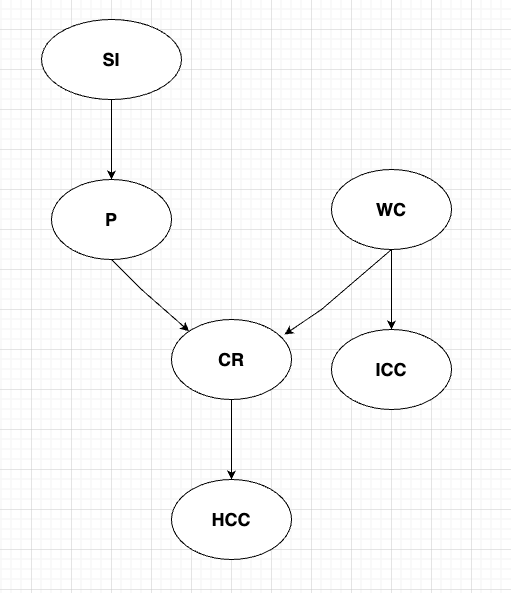
\includegraphics[width=0.5\textwidth]{image.png}
    \caption{Visual representation of the Bayesian network}
    \label{fig:your_label}
\end{figure}


\subsection*{b)}

There is no casual independence between ice cream consumption and home security systems since there is no direct relation between these two events. Casual indepence can be mentioned only on direct relations. 

However, there is a statistical dependence between these two nodes. There share a common cause, which is warm climate.

\section*{Question 2}

\subsection*{a)}

We can find this probability buy finding the both probabilities where lung disase is true or false.

\[
    P(x_1, x_2, \dots x_n) = \prod_{i=1}^{n} P(x_i \mid \text{Parents}(X_i))
\]

\begin{align*}
P(SB|S) \wedge P(CP|S) &= P(SB|LD=T) \cdot P(CP|LD=T) \cdot P(LD=T|S) \\
&\quad + P(SB|LD=F) \cdot P(CP|LD=F) \cdot P(LD=F|S) \\
&= (0.208) \cdot (0.208) \cdot (0.101) + (0.01) \cdot (0.01) \cdot (0.899) \\
&= 0.004 + 0.000 \\
&= 0.004
\end{align*}


\subsection*{b)}

Firstly, calculating necessary Bayesian probabilities:

\begin{itemize}
    \item $P(LD=T) = (0.101) \cdot (0.2) + (0.001) \cdot (0.8) = 0.021$
    \item $P(CO=T | LD=T) = (0.753) \cdot (0.02) + (0.505) \cdot (0.98) = 0.51$
    \item $P(CO=T | LD=F) = (0.505) \cdot (0.02) + (0.01) \cdot (0.98) = 0.02$
\end{itemize}

Using Bayes' Rule to find the final probability:
\begin{align*}
P(LD=T | CO=T) &= \frac{P(CO=T | LD=T) \cdot P(LD=T)}{P(CO=T)} \\    
P(LD=T | CO=T) &= \frac{P(CO=T | LD=T) \cdot P(LD=T)}{P(CO=T | LD=T)P(LD=T) + P(CO=T | LD=F)P(LD=F)} \\
&= \frac{0.51 \cdot 0.021}{(0.51 \cdot 0.021) + (0.02 \cdot 0.979)} \\
&= \frac{0.011}{0.011 + 0.02} = {0.355}
\end{align*}

\subsection*{c)}

We can find this probability by first calculating the probability of having a cold given fever, and then using that to find the cough probability for the person with lung disease.

\begin{itemize}
    \item $P(F=T) = (0.307) \cdot (0.02) + (0.01) \cdot (0.98) = 0.016$
    \item $P(C=T | F=T) = \frac{0.307 \cdot 0.02}{0.016} = 0.383$
    \item $P(C=F | F=T) = \frac{0.01 \cdot 0.98}{0.016} = 0.612$
    \item $P(LF) = P(LD=T) \cdot P(F=T) = (0.021) \cdot (0.016) = 0.000336$
\end{itemize}

LF variable is the joint probability of having lung disease and fever.

\begin{align*}
P(CO=T \mid LF=T) &= \frac{P(CO=T, LF=T)}{P(LF)} \\
&= P(CO=T \mid LD=T, C=T) \cdot P(C=T \mid F=T) + P(CO=T \mid LD=T, C=F) \cdot P(C=F \mid F=T) \\
&= (0.753) \cdot (0.383) + (0.505) \cdot (0.612) \\
&= 0.288 + 0.309 = {0.597}
\end{align*}

\subsection*{d)}

We can find this probability by finding both probabilities where lung disease is true or false given that the person smokes, and then normalizing. We use $SCP$ to represent the probability of having chest pain given the smoking status.

\begin{itemize}
    \item $P(LD=T | S=T) = 0.101$
    \item $P(LD=F | S=T) = 0.899$
    \item $P(SCP) = P(CP=T | S=T) = (0.208) \cdot (0.101) + (0.01) \cdot (0.899) = 0.03$
\end{itemize}

\begin{align*}
P(LD=T | S=T, CP=T) &= \frac{P(CP=T | LD=T) \cdot P(LD=T | S=T)}{P(SCP)} \\
&= \frac{0.208 \cdot 0.101}{0.03} \\
&= \frac{0.021}{0.03} = {0.7}
\end{align*}

\subsection*{e)}

We can find this probability by finding both probabilities where lung disease is true or false given that the person does not have a cold. We use NCCO to represent the probability of having a cough given that the person has no cold.

\begin{itemize}
    \item $P(LD=T) = 0.021$
    \item $P(LD=F) = 0.979$
    \item $P(NCCO) = P(CO=T | C=F) = (0.505) \cdot (0.021) + (0.01) \cdot (0.979) = 0.02$
\end{itemize}

\begin{align*}
P(LD=T | CO=T, C=F) &= \frac{P(CO=T | LD=T, C=F) \cdot P(LD=T)}{P(NCCO)} \\
&= \frac{0.505 \cdot 0.021}{0.02} \\
& = {0.53}
\end{align*}

\subsection*{f)}

We can find this probability by calculating the joint probability of the symptoms given the smoking status, and then normalizing. We use $SBCO$ to represent the total probability of having both shortness of breath and a cough.

\begin{itemize}
    \item $P(SB, CO | S=T) = (0.208 \cdot 0.51) \cdot 0.101 + (0.01 \cdot 0.02) \cdot 0.899 = 0.011$
    \item $P(SB, CO | S=F) = (0.208 \cdot 0.51) \cdot 0.001 + (0.01 \cdot 0.02) \cdot 0.999 = 0.0003$
    \item $P(SBCO) = (0.011) \cdot (0.2) + (0.0003) \cdot (0.8) = 0.00244$
\end{itemize}

\begin{align*}
P(S=T | SB=T, CO=T) &= \frac{P(SB, CO | S=T) \cdot P(S=T)}{P(SBCO)} \\
&= \frac{0.011 \cdot 0.2}{0.00244} \\
&= \frac{0.0022}{0.00244} = {0.902}
\end{align*}

\end{document}
